\section{Auswertung}

Bevor wir das SQUID eingeschaltet haben, haben wir die Distanz der Probe zum SQUID-Sensor gemessen. Diese beträgt:

$$z = (3,6 \pm 0,2)\ cm$$

Nach dieser Messung haben wir den flüssigen Stickstoff in das Kryostat gefüllt und den SQUID-Sensor eingefügt. Wir haben 15 Minuten gewartet, und dann mit der Justierung begonnen.

\subsection{Justierung des SQUIDs}

Die Justierung des SQUIDs haben wir anhand des Programms \emph{JSQ Duo Sensor Control} an einem PC und einem Oszilloskop durchgeführt. Wir haben die Software in den Test-Modus geschaltet, welcher einen Funktionsgenerator dazu veranlasst, eine Dreieckspannung in den Schwingkreis einzukoppeln. Diese beeinflusst dann die Spannungsantwort des SQUID, die wir am Oszilloskop einsehen können, das sogenannte \emph{SQUID-Pattern}. Zum Triggern schließen wir dann den Funktionsgenerator noch direkt an den Oszilloskop.  Dann haben wir den Arbeitspunkt anhand der Software justiert, sodass die Amplitude des SQUID-Patterns maximal wurde. Unsere Einstellparameter lauten:\\

\begin{center}
\begin{tabular}[H]{l l}
	$VCA = 1391$ & Stromamplitude des Schwingkreises ($\sim 6\cdot 10^{-8} W$)\\
	$VCO = 1477$ & Frequenz des Schwingkreises ($\sim 760 MHz$)\\
	$OFF = 1471$  & Offset des Signals
\end{tabular}
\end{center}

\begin{figure}[H]
	\centering 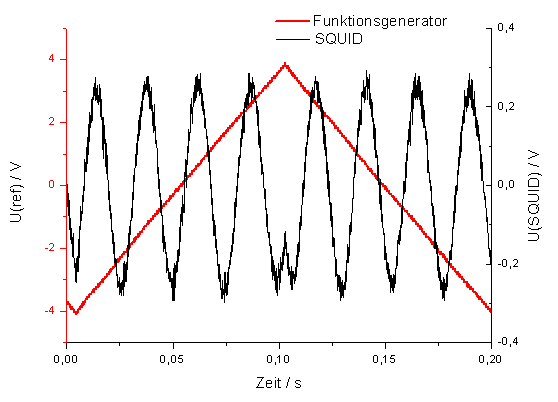
\includegraphics[width = 0.78\textwidth]{Bilder/Pattern1.png}
	\caption{Das SQUID-Pattern}
\end{figure}

\subsection{Dipolmoment und Magnetfeldstärken der Leiterschleife}

\subsubsection{Berechnung}

Wir haben eine stromdurchflossene Leiterschleife mit Durchmesser $d = (3,5 \pm 0,3)\ mm$ am SQUID für 5 verscheide Widerstände gemessen. Aus dem gemessenen Durchmesser ergibt sich der Radius $r=d/2$ mit Fehler $s_r = s_d/2$: $$r = (1,75 \pm 0,15) mm$$

Das magnetische Dipolmoment berechnen wir mit der Formel:

$$p = I\cdot A = \frac{U}{R}\pi r^2 \text{ \ \ \ mit \ \ \ } s_p = p\sqrt{\frac{s_U^2}{U^2} + \frac{s_R^2}{R^2} + 2\frac{s_r^2}{r^2}}$$

Die Feldstärke berechnen wir mit der Formel:

$$B = \frac{\mu_0}{2\pi}\frac{p}{z^3} \text{ \ \ \ mit \ \ \ } s_B=B\sqrt{\frac{s_p^2}{p^2} + 3 \frac{s_z^2}{z^2}}$$

Wir erhalten die Werte:

\begin{figure}[H]
	\centering 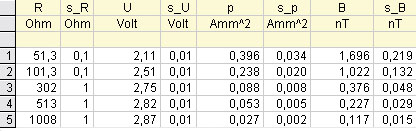
\includegraphics{Bilder/Tab-Leiterschleife.jpg}
\end{figure}

\subsubsection{Graphisch}

























